\chapter{Marco Metodológico}

\section{Tipo de Estudio}
El tipo de estudio es hipotético deductivo, cuantitativo.

Es hipotético deductivo porque:

\begin{itemize}
\item partimos de una teoría base (macroeconomía que sustenta la tasa de cambio con la balanza de pagos y exportaciones, machine learning para deducir modelos predictivos en base a grandes muestras de datos) formulamos una hipótesis de trabajo
\item aplicamos ciencia de datos para una recolección masiva de datos de diferentes regresores (cada uno un rubro importante de exportaciones de Colombia)
\item Confirmamos la hipótesis al extraer un modelo predictivo estadístico  
\end{itemize}

\subsection{Metodología de Estudio}
Enfoque cuantitativo experimental utilizando Machine Learning.

\begin{itemize}
	\item Método ensamblado de GLM y ARIMA
	\item Aprendizaje automatizado
	\item Biblioteca CARET para la creación de muestras aleatorias de entrenamiento y evaluación cruzada
	\item 70\% datos de entrenamiento
	\item 30\% datos de evaluación cruzada
\end{itemize}
    
\subsection{Impacto Social}
El trabajo cumple con la dimensión de relevancia social. Ninguna empresa quiere costear sus productos por encima de los demás agentes del mercado, so pena de perder participación de mercado a sus competidores con precios más ventajosos. La capacidad de estimar a futuro el mejor pronóstico de tasa de cambio reduce el porcentaje de carga por previsión de volatilidad de moneda (también conocido en contabilidad como colchón) lo que redunda en un precio mejor para el consumidor y la sociedad en general. Al reducir las ineficiencias del cálculo de costos prediciendo de forma correcta la tasa de cambio los consumidores ganan el diferencial entre el precio pobremente estimado y un precio ajustado a las realidades del cambio futuro.

\section{Descripción del Método}
La metodología utilizada para el trabajo de investigación se apega estrictamente a la formalización de la hipótesis de trabajo:

\[ p^{c}(x) = (p^{c}(c_{1} \mid x),p^{c}(c_{2} \mid x)) \]

Donde:

\[ c_{1} : f(y) = \beta_{0} + \beta_{1}x_{1} + \beta_{2}x_{2} + \cdots + \beta_{n}x_{n} + \epsilon \]
\[ c_{2} : f(y_{t}) = \beta_{0} + \beta_{1}x_{t-1} + \beta_{2}x_{t-2} + \cdots + \beta_{n}x_{t-n} + \epsilon_{t}\]

Por lo tanto la metodología del estudio se puede resumir en un método ensamblado de aprendizaje automatizado resultante de la composición de dos aprendices: uno basado en un regresor lineal y el segundo basado en un pronostico ARIMA. Los valores estimados para cada caso del arreglo de datos se utilizan como variable independiente y predictor del modelo ensamblado, con la variable dependiente inmutable. El modelo ensamblado entonces se entrena nuevamente con los resultados de las predicciones contra los valores reales.   

Podemos resumir el proceso con el siguiente esquema de arquitectura del modelo:\\

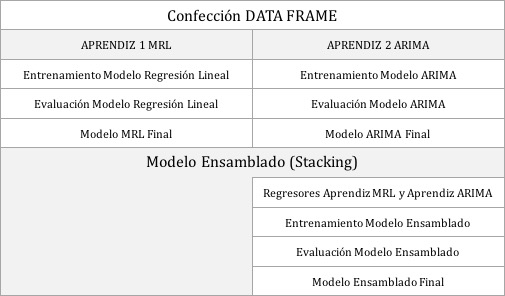
\includegraphics[width=\textwidth]{ArquitecturaModeloEnsamblado}\\

Cada aprendiz es a su vez un modelo de aprendizaje automatizado con su propia metodología de investigación. 

\subsubsection{Aprendiz 1: Modelo de Regresión Lineal}
\begin{itemize}
	\item El aprendiz 1 es un modelo de regresión lineal utilizando como variable dependiente el valor de la TRM para cada día del juego de datos y como regresores un arreglo asociado de cotizaciones del precio promedio mundial de los once productos principales de la canasta de exportación de Colombia entre los años 2010 y 2017.
	\item Para el juego de entrenamiento se selecciona un 70\% de los datos disponibles. Dicha selección se hace con la ayuda de la biblioteca CARET de R para funciones de aprendizaje automatizado. 
	\item Para el juego de validación se selecciona un 30\% de los datos disponibles. Dicha selección también se hace con la ayuda de la biblioteca CARET de R para funciones de aprendizaje automatizado. 
	\item La variable SEED se prefigura al valor arbitrario \emph{7556014} para propósitos de reproducibilidad de los datos. 
	\item El aprendizaje automatizado no asegura que todos los regresores sean útiles o necesarios para una predicción dentro de los valores de confianza esperados. Existe la posibilidad que un número limitado de regresores cumpla con los mismos valores de predicción que la totalidad de los mismos y que el modelo generalice mejor al tener menos regresores (disminuyendo la inflación de la varianza como efecto secundario). 
	\item Para determinar el número óptimo de regresores se procedió a armar el modelo de aprendizaje automatizado sumando un regresor a la vez y analizando los valores del coeficiente de determinación y coeficiente de correlación. Los valores finales del error mínimo cuadrático de cada modelo se comparan para determinar la mejor combinación de regresores. 
	\item Como segunda validación para la combinación correcta de regresores, se utilizó el análisis \emph{Step\_AIC} (reducción óptima de regresores utilizando análisis combinatorio y el Criterio de Información de Aikake) con la biblioteca \emph{STEP\_AIC} de \emph{R}. El método \emph{STEP\_AIC} es intensivo en recursos de computación y no siempre arroja resultados superiores a los que un investigador pueda armar a mano utilizando técnicas visuales de exploración de datos.
\end{itemize}

\subsubsection{Aprendiz 2: Modelo ARIMA}
\begin{itemize}
	\item El aprendiz 2 es un modelo de pronostico ARIMA utilizando como serie de tiempo el valor de la TRM para cada día del juego de datos entre los años 2010 y 2017.
	\item Para el juego de entrenamiento se selecciona un 70\% de los datos disponibles. Dicha selección se hace con la ayuda de la biblioteca FORECAST de R para funciones de aprendizaje automatizado utilizando series de tiempo \cite{hyndman}. 
	\item Para el juego de validación se selecciona un 30\% de los datos disponibles. Dicha selección también se hace con la ayuda de la biblioteca FORECAST de R para funciones de aprendizaje automatizado de series de tiempo. 
	\item La variable SEED se prefigura al valor arbitrario \emph{7556014} para propósitos de reproducibilidad de los datos. 
\end{itemize}

\subsubsection{Clasificador Ensamblado}
\begin{itemize}
	\item El clasificador ensamblado se toma como un arreglo de una variable dependiente (el valor de la TRM para cada día correspondiente al juego de datos) y dos variables independientes (los resultados de la predicción de los dos aprendices). 
	\item Para el juego de entrenamiento se selecciona un 70\% de los datos disponibles. Dicha selección se hace con la ayuda de la biblioteca CARET de R para funciones de aprendizaje automatizado. 
	\item Para el juego de validación se selecciona un 30\% de los datos disponibles. Dicha selección también se hace con la ayuda de la biblioteca CARET de R para funciones de aprendizaje automatizado. 
	\item La variable SEED se prefigura al valor arbitrario \emph{7556014} para propósitos de reproducibilidad de los datos. 
	\item El modelo se resuelve utilizando la metodología de Stacking como un modelo de regresión lineal (Smolyakov, V., 2017 y Opitz, D. y Maclin, R., 1999).
\end{itemize}

\subsubsection{Validación del Modelo Ensamblado}
Se espera del modelo final un nivel de desempeño con predicciones dentro de un \(\alpha \leq 0.05\). Para tal fin dentro del diseño de investigación se valida el modelo sometiendo el mismo a un juego aleatorio de 100 datos de muestra que comprende:

\begin{itemize}
	\item Resultados de predicción del modelo versus el modelo aprendiz 1 de regresión lineal multivariable.
	\item Resultados de predicción del modelo ensamblado versus el modelo aprendiz 2 ARIMA. 
	\item Resultados de predicción del modelo ensamblado versus un intervalo de confianza del 99\%.
\end{itemize}

El modelo se considera óptimo para producción si pasa las tres pruebas de validación.  

\section{Diseño de la Instrumentación}
\subsection{Componentes de Investigación Series de Tiempo}
Un componente de aportación es cualquier rubro que se supone se exporta desde Colombia, aporta ingresos en dólares, y por lo tanto ayuda a equilibrar la balanza de pagos y demanda demanda de divisas - y por ende la TRM. Es importante hacer un análisis de cada uno de estos que debe incluir \cite{zumelMount}:

\begin{itemize}
	\item carga inicial como serie de tiempo (time series class)
	\item start(), end()
    \item summary()
    \item plot.ts()
    \item acf()
    \item pacf()
    \item descomponer en stl()
    \item prueba Dickey Fuller adf.test()
\end{itemize}

\subsection{Análisis de Componente de Aportación}

\subsubsection{Carga Inicial de Datos}
La carga inicial de datos para el precio internacional del café se hace a través del servicio web de Quandl.

\begin{lstlisting}[language=R]
# Load coffee prices as time series
library(Quandl)
library(tseries)

Quandl.api_key("KzzS8Vfxkw1ZgTWgU4jH")
coffee <- Quandl("ODA/PCOFFOTM_USD", collapse = "monthly", type = "ts")
head(coffee)
class(coffee)
cycle(coffee)
\end{lstlisting}

\subsection{EDA (Explorative Data Analysis)}
La forma más sencilla de ver los efectos del precio del café es revisar la tendencia del precio internacional y revisar si ha habido efectos por temporada o alguna tendencia \cite{daroczi}.

\begin{lstlisting}[language=R]
plot.ts(coffee)
abline(reg = lm(coffee ~ time(coffee)))
\end{lstlisting}

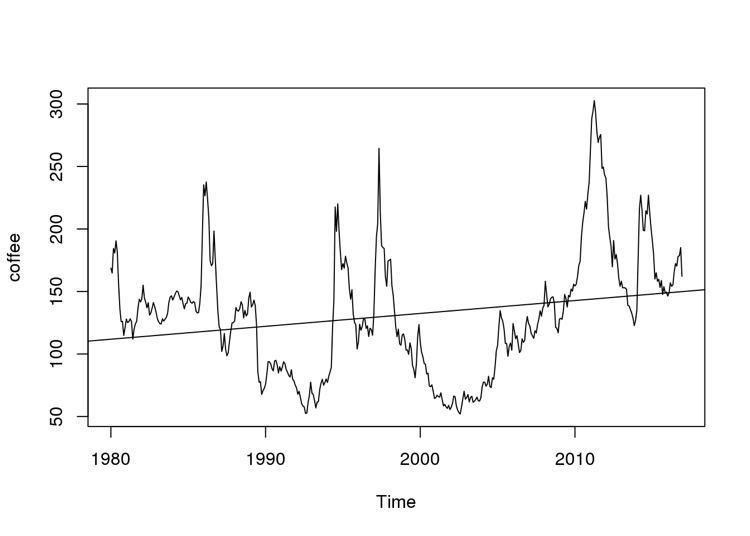
\includegraphics[width=\textwidth]{correlacionTiempoCafe}\\

Otro examen necesario es el de autocorrelación y autocorrelación parcial. Ambos análisis nos permiten ver si la serie es del tipo auto-regresiva o de promedios móviles \cite{hyndman}.

\begin{lstlisting}[language=R]
par(mfrow=c(1,2))
acf(coffee)
pacf(coffee)
\end{lstlisting}

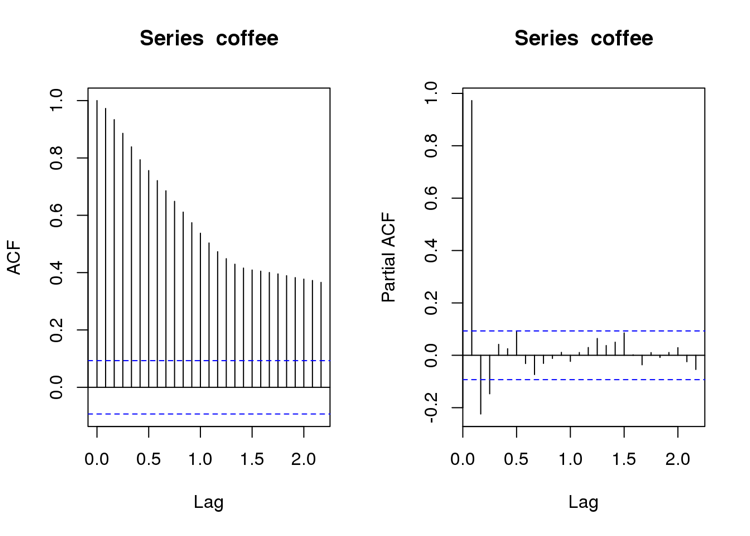
\includegraphics[width=\textwidth]{autocorrelacion}\\

El último examen es la descomposición de la serie en datos, temporalidad y tendencia, para ver si alguno de estos elementos está presente.

\begin{lstlisting}[language=R]
decomp <- stl(coffee, s.window = 11)
plot(decomp)
\end{lstlisting}

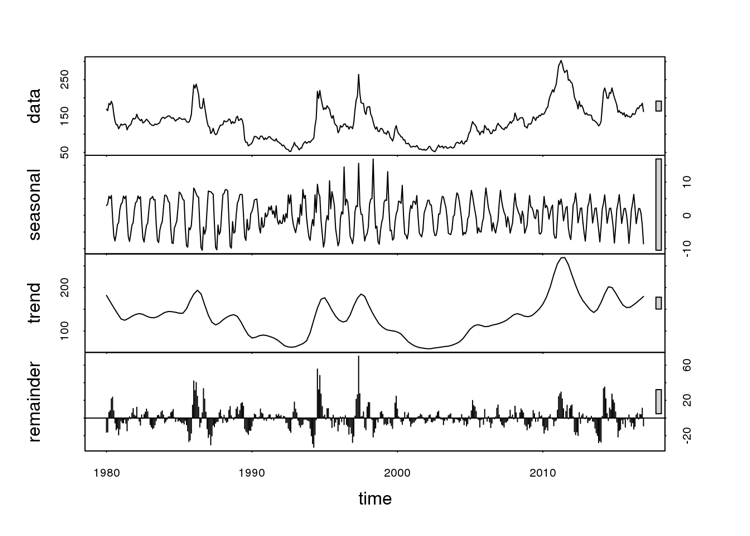
\includegraphics[width=\textwidth]{decopSTLCafe}\\

\subsection{Dickey Fuller Test para Series Temporales}
El test \emph{Dickey Fuller} \cite{dickeyfuller} es la prueba mas importante para la verificación de la estacionalidad de una serie de tiempos. La literatura recomienda altamente someter todas las pruebas de series al test \emph{Dickey Fuller} antes de proceder con otros análisis \cite{hyndman}.

\begin{lstlisting}[language=R]
# Dickey Fuller Test for stationary time series
df <- adf.test(coffee, k = 12)
df$statistic
df$p.value
\end{lstlisting}

\section{Regresión Lineal con Calce de la Función de Predicción}
Los modelos de regresión lineal utilizan la biblioteca \emph{Quandl} para la extracción de datos y deben hacer la transformación del arreglo de datos a una serie de tiempos. Los datos serán colapsados de forma mensual y se revisará la fórmula de la función de calce para el coeficiente de correlación y determinación \cite{narayanachar}. 

\begin{lstlisting}[language=R]
# Load oil prices as time series
library(Quandl)
library(tseries)

Quandl.api_key("KzzS8Vfxkw1ZgTWgU4jH")
wti <- Quandl("EIA/PET_RWTC_D", collapse = "monthly", type = "ts")
head(wti)
class(wti)
cycle(wti)

plot.ts(wti)
abline(reg = lm(wti ~ time(wti)), col="red")
fit = lm(wti ~ time(wti))
summary(fit)


Call:
lm(formula = wti ~ time(wti))

Residuals:
    Min      1Q  Median      3Q     Max 
-45.031 -13.929  -0.368  11.399  80.925 

Coefficients:
              Estimate Std. Error t value Pr(>|t|)    
(Intercept) -4849.3862   213.2634  -22.74   <2e-16 ***
time(wti)       2.4439     0.1065   22.94   <2e-16 ***
---
Signif. codes:  0 '***' 0.001 '**' 0.01 '*' 0.05 '.' 0.1 ' ' 1

Residual standard error: 19.43 on 384 degrees of freedom
Multiple R-squared:  0.5782,	Adjusted R-squared:  0.5771 
F-statistic: 526.4 on 1 and 384 DF,  p-value: < 2.2e-16
\end{lstlisting}

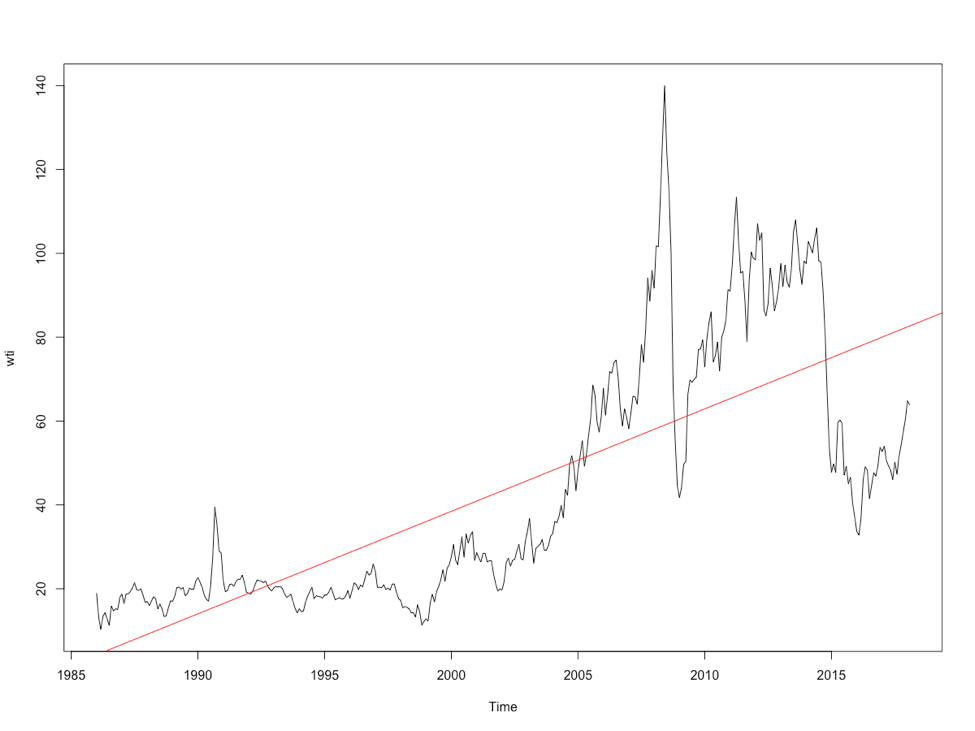
\includegraphics[width=\textwidth]{regresionTiempoWTI}\\

\subsubsection{Modelo Predictivo Ensamblado} 
El modelo predictivo ensamblado es el resultado del entrenamiento de un modelo predictivo de regresión lineal y un modelo ARIMA. Ambos modelos se combinan y se entrenan con la variable de valor real en común para ambos \cite{viswanathan}.

\begin{lstlisting}[language=R]
# Pseudo-codigo R simplificado
# Funcion de modelo ensamblado

# Cargar Data Frame con informacion de series de tiempo
library(caret)
set.seed(7556014)
data(featuresTRM)
data(TRM)
adData = data.frame(TRM, featuresTRM)
inTrain = createDataPartition(adData$TRM, p = 3/4)[[1]]
training = adData[ inTrain,]
testing = adData[-inTrain,]

set.seed(7556014)

modelo1 <- train(TRM ~ ., method = "glm", data = training)
modelo2 <- train(TRM ~ ., method = "ARIMA", data = training)

# Vectores de valores de prediccion de cada modelo
predVec1 <- predict(modelo1, testing)
predVec2 <- predict(modelo2, testing)

# Construccion de matriz de datos ensamblados (variable dependiente y predictor)
predDF <- data.frame(TRM = testing$TRM, predVec1, predVec2)

# Modelo combinado (fit)
combModelFit <- train(TRM ~ ., method = "glm", data = predDF)
finalPred <- predict(combModelFit, predDF) 
\end{lstlisting}

\section{Diseño de muestreo}

\subsection{Introducción al Cálculo de la Muestra del Proyecto de Investigación}
Inicialmente, podemos calcular el tamaño de la muestra necesaria para nuestro estudio con la fórmula (Mendenhall, W., Beaver, R. y Beaver, B., 2010):

\[ n =  (N* z^2*p*q)/(E^2*(N-1)+ z^2*p*q)\]

El tamaño total de todas las cotizaciones de la TRM o del precio internacional del petróleo WTI es un número finito. Los mercados funcionan de lunes a viernes, por lo general las cincuenta y dos semanas del año, por lo que el número total de posibles cotizaciones oficiales en un año dado cualesquiera se determinan como:

\[N_regresor=numero_semanas_years*dias_semana_laboral\]

La fórmula es muy simple y equivale a sustituir cualquier variable regresor (por ejemplo, el valor del petróleo WTI) por los números reales de días laborales y semanas del año. 

\[N_wti=52*5=260\]

Ende, existen 260 posibles valores de la cotización del petróleo WTI en un año cualesquiera. Dado que el modelo de predicción de aprendizaje automatizado utiliza datos del año 2010 al 2017 inclusive, podemos ampliar el universo dentro del período de estudio con la siguiente formula:

\[N_regresorPeriodoEstudio=numero_(semanas_year )*dias_(semana_laboral )*years\]

El cual se resuelve como:

\[N_wtiPeriodoEstudio=52*5*8=2,080\]

Nuestro universo por regresor equivale a dos mil ochenta puntos de datos. Para un estudio con un nivel de confianza del 99\% y un error de estimación del 5\% calculamos el número de la muestra como una proporción, donde:

\begin{align*}
  N =& 2,080 {puntos de datos} \\
  p =& 0.5 \\
  q =& 0.5 {o} (1 – p) \\
  z =& 99\% {o 2.575} \\
  e =& 5\% {\approx 0.05} \\
\end{align*}

Utilizamos el lenguaje R para resolver el cálculo:

\begin{lstlisting}[language=R]
N <- 2080
p <- 0.5
q <- 1 - p
z <- 2.575
E <- 0.05

muestra <- (N * z^2 * p * q) / ((N - 1) * E^2 + z^2 * p * q)
muestra
[1] 502.9681
\end{lstlisting}

El tamaño de la muestra es 503 puntos de datos por regresor a utilizar. Sin embargo, dado que los usos de técnicas de Ciencia de Datos nos permiten acceder a la biblioteca Quandl de forma de recolectar el universo entero de datos, utilizaremos los 2,080 puntos de datos para cada regresor, trabajando de esta forma con el universo entero y no la muestra. Este es un buen ejemplo del uso de Big Data (Peng, 2014) que no solo aplica a muestras grandes de universos extensos, sino al total de la data de un universo pequeño. 

\subsubsection{Observaciones Adicionales Sobre el Uso de Muestras dentro de Diseños de Investigación con Regresión Lineal}
No todos los autores están de acuerdo con el uso de la fórmula tradicional para el cálculo del número de muestras en un estudio de regresión lineal. William Dupont y Walton Plummer han discutido el uso de técnicas alternativas cuando los estudios (sobre todo los estudios clínicos) utilizan regresiones lineales multivariable (Dupont, W. y Plummer, W., 1998). Dichas técnicas se apoyan en la identificación de diferentes pendientes en los análisis de regresión versus el uso de coeficientes (argumentando que es más fácil comparar visualmente pendientes versus coeficientes) y el manejo del poder estadístico $1 – \beta$. Sobre este último los autores manifiestan ajustar los niveles de poder para verificar en que momento del cambio se detecta diferencias de la pendiente de una hipótesis contra su hipótesis alternativa dentro de una muestra de n pacientes. 

Al momento de preparar el diseño del estudio, las herramientas de medición y la muestra, el doctorando ha decidido no profundizar más en métodos menos tradicionales de cálculo de muestras en estudios de regresión lineal, dado que en el caso específico se utilizará la totalidad del universo, haciendo el cálculo de muestra innecesario. 

\section{Trabajo de campo (laboratorio)}

